\documentclass[10pt,letterpaper]{article}
\usepackage[letterpaper, margin=2cm]{geometry}
\usepackage{graphicx,amsmath,verbatim,textcomp,amssymb,bm,enumerate,fontenc,graphicx,titling,cmbright,mathtools,tikz}
\usepackage[OT1]{fontenc}

\begin{document}	
	
	\setlength{\droptitle}{-2cm}
	
	\title{ \textbf{USAD Mathematics Reference} }
	\author{ \textit{Created for the Lane Tech ACADEC Team} }
	\date{ \textit{2025-2026} }
	
	\maketitle
	
	\normalfont
	
	\section{Introduction}
	
	\begin{enumerate}
		
		\item[] 
		This Reference will cover a variety of topics and mathematical rules that are often need of additional practice to better succeed at USAD Competitions. The first part of this Reference will elaborate on various basic mathematics concepts, ideas, complete with supplementary visuals.
		\vskip 10pt
		The second part of this Reference will go over, solve, and explain questions commonly found on USAD\\ Mathematics exams, approaches to these questions, and a variety of methods and explanations as to how these solutions work. Figures and supplementary text, along with step-by-step solutions to practice problems, will be provided. Any concepts at greater than an Advanced Algebra level will be explained.
		
	\end{enumerate}
	
	\section{Useful Mathematics Concepts, Rules, and Identities}
	
		\subsection{Radians, Degrees and the Unit Circle}
		
		\begin{enumerate}
			\item 
			
			Two mathematical systems are used to describe a given angle : degrees and radians.
			
			\begin{enumerate}
				\item 
				
				The degree system divides one full rotation into 360 degrees.
				
				\item 
				
				The radian system divides one full rotation into 2$\pi$.
				
				\item
				
				Both systems employ a 'standard angle reference' on the unit circle, which is the positive X axis.
				
			\end{enumerate}
			
		\item
		
		Below is the unit circle. The first value is the angle from the 'standard reference angle' in degrees, radians and then the coordinate location of that angle's intersection with the circumference of the circle.
			
		\end{enumerate}
			
			\begin{center}
			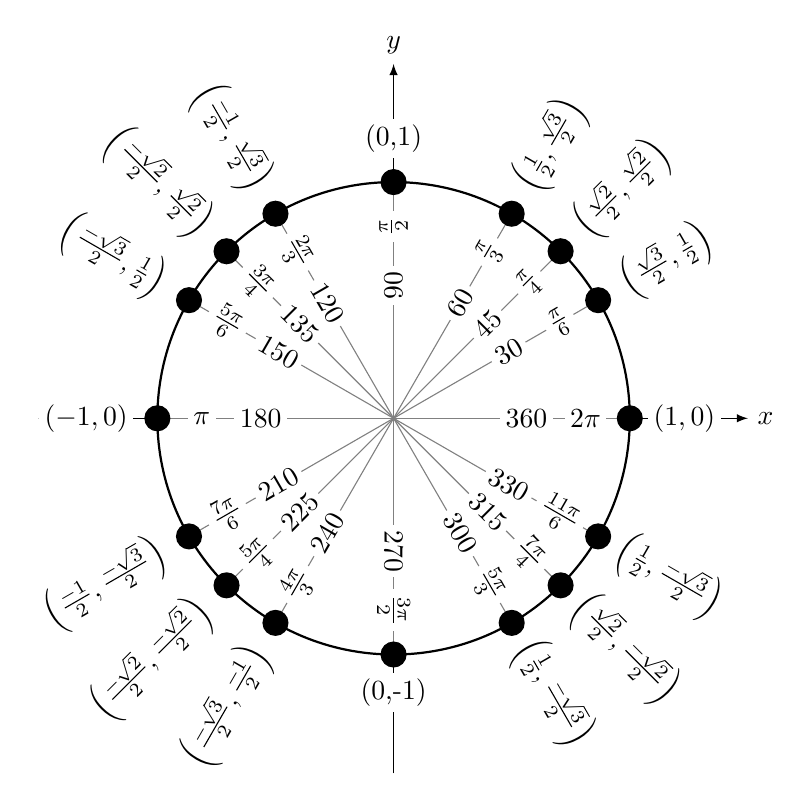
\begin{tikzpicture}[scale=3,
			cap = round,
			> = latex,
			dot/.style = {circle, fill, minimum size=0.5mm},
			lbl/.style = {fill=white, inner sep=2pt, near start, sloped}
			]
			% draw the coordinates
			\draw[->] (-1.5,0) -- (1.5,0) node[right] {$x$};
			\draw[->] (0,-1.5) -- (0,1.5) node[above] {$y$};
			% draw the unit circle
			\draw[thick] (0,0) circle[radius=1];
			% draw dots, labels
			\foreach \i/\j/\k in {
				30/\frac{\pi}{6}/{\left(\frac{\sqrt{3}}{2},\frac{1}{2}\right)},
				45/\frac{\pi}{4}/{\left(\frac{\sqrt{2}}{2},\frac{\sqrt{2}}{2}\right)},
				60/\frac{\pi}{3}/{\left(\frac{1}{2},\frac{\sqrt{3}}{2}\right)},
				90/\frac{\pi}{2}/{\rotatebox{-90}{(0,1)}},
				120/\frac{2\pi}{3}/{\left(\frac{-1}{2},\frac{\sqrt{3}}{2}\right)},
				135/\frac{3\pi}{4}/{\left(\frac{-\sqrt{2}}{2},\frac{\sqrt{2}}{2}\right)},
				150/\frac{5\pi}{6}/{\left(\frac{-\sqrt{3}}{2},\frac{1}{2}\right)},
				180/\pi/{(-1,0)},
				210/\frac{7\pi}{6}/{\left(\frac{-1}{2},\frac{-\sqrt{3}}{2}\right)},
				225/\frac{5\pi}{4}/{\left(\frac{-\sqrt{2}}{2},\frac{-\sqrt{2}}{2}\right)},
				240/\frac{4\pi}{3}/{\left(\frac{-\sqrt{3}}{2},\frac{-1}{2}\right)},
				270/\frac{3\pi}{2}/{\rotatebox{90}{(0,-1)}},
				300/\frac{5\pi}{3}/{\left(\frac{1}{2},\frac{-\sqrt{3}}{2}\right)},
				315/\frac{7\pi}{4}/{\left(\frac{\sqrt{2}}{2},\frac{-\sqrt{2}}{2}\right)},
				330/\frac{11\pi}{6}/{\left(\frac{1}{2},\frac{-\sqrt{3}}{2}\right)},
				360/2\pi/{(1,0)}
			}
			{
				\path[draw=gray]    (\i:0) -- (\i:0.5)
				-- node[lbl] {$\i$} (\i:0.75)
				-- node[lbl] {$\j$} (\i:1) node[dot] {};
				\ifnum\i<270
				\ifnum\i>90
				\path   (\i:1) --  node[lbl, anchor=east] {$\k$} (\i:1.4);
				\else
				\path   (\i:1) --  node[lbl, anchor=west] {$\k$} (\i:1.4);
				\fi
				\else
				\path   (\i:1) --  node[lbl, anchor=west] {$\k$} (\i:1.3);
				\fi
			}
			
		\end{tikzpicture}
		\end{center}
		
		\subsection{Right Triangle Relationships}
		
%		\includegraphics[scale=0.3]{"../Pictures/Screenshots/Screenshot from 2026-01-14 14-42-26"}
		
		\begin{enumerate}
			\item 
			
			In the right triangle above, the capital letters represent the angle which they are adjacent, and the lowercase letters sides. Your knowledge of \textit{"SOH CAH TOA"} is assumed.
			
			In a right triangle, such as shown above, the following identities hold true :
				
				\begin{equation}
					\sin(A) = \cos(B) = \frac{a}{c}
				\end{equation}

				\begin{equation}
					\cos(A) = \cos(B) = \frac{b}{c}
				\end{equation}

				\begin{equation}
					\tan(A) = \cot(B) = \frac{a}{b}
				\end{equation}
				
				\begin{equation}
					\cot(A) = \tan(B) = \frac{b}{a}
				\end{equation}

		\end{enumerate}
		
		\subsection{Useful Equations}
		
		\begin{enumerate}
			\item Circle Equation
			
			The equation for a circle is as follows, where r is the radius of the circle, a is the horizontal offset and b is the vertical offset from (0,0):
				
			\begin{equation}
				r^2 = (x+a)^2 + (y+b)^2
			\end{equation}
			
			\item Heron's Formula
			
			Heron's formula allows you to solve for the area of any triangle with 3 given sides, \textit{a, b} and \textit{c}, using the semiperimeter of the triangle, which is defined as half the perimeter.
			
			\begin{equation}
				A = \sqrt{s(s-a)(s-b)(s-c)}
			\end{equation}
			
		\end{enumerate}
		
		\subsection{Rational Root Theorem}
		
		\subsection{Dot Products}
		
		\begin{enumerate}
			
			
			\item 
			
			Given two lines of the following equations, find the angle between these two lines using the dot product method.
			
			\begin{equation}
				y = \frac{3}{2}x + 2
			\end{equation}
			
			\begin{equation}
				y = \frac{5}{3} x + 4
			\end{equation}
			
			\item 
			
			Vectors take the form of $\langle$ x,y $\rangle$, where x is the direction and y is the magnitude. We can convert the slopes of these equations above into vectors which we can then extract the angle from using the dot product of these two vectors.
	
			\item 
		
			Slopes are represented as $\frac{\Delta y}{\Delta x}$, or the change in (delta of) x over the change in y.
			
			\item
			
			We can convert these slopes ($\frac{3}{2}$ and $\frac{5}{3}$, respectively) into vectors simply by putting in the $\Delta$x as x in the vector and $\Delta$y as y in the vector. Doing this, we get the vectors :
			
			\begin{equation}
				\langle 2,3 \rangle
			\end{equation}
			
			\begin{equation}
				\langle 3,5 \rangle
			\end{equation}
			
			\item 
			
			With these vectors, we can calculate their dot product. To manually calculate the dot product, you must perform the following :
			
			\begin{equation}
				x_1x_2 + y_1y_2 = s
			\end{equation}
			
			Plugging in our vector values, it looks like this :
			
			\begin{equation}
				2(3) + 3(5) = s = 21
			\end{equation}
			
			\item 
			
			This scalar, denoted as s, is the dot product, but it is not the resulting angle yet. We must perform a few more operations. The resultant angle is equal to :
			
			\begin{equation}
				s = \sqrt{x_1^2+y_1^2}\sqrt{x_2^2+y_2^2}\cos\theta
			\end{equation}
			
			Plugging in our values, we get this :
			
			\begin{equation}
				21 = \sqrt{2^2+3^2}\sqrt{3^2+5^2}\cos\theta
			\end{equation}
			
			\item 
			
			After evaluating for $\theta$, we get 
			
			\begin{equation}
			\arccos\frac{21}{\sqrt{2^2+3^2}\sqrt{3^2+5^2}} = \theta
			\end{equation}
			
			\begin{equation}
				\theta \approx 2.72^\circ
			\end{equation}
			
		\end{enumerate}
	
		\subsection{Properties of Logarithms}
		
		
		
		\begin{comment}
			
			
		LAW OF COSINES
		
		an triangle (doesnt have to be right) finding angle B
 /m		======		a & c sides interchangeable (see above)
		
		a^2 = b^2 + c^2 - 2bc * cos(B)
		
		LAW OF SINES
		
		sinA/a = sinB/b * sinC/c
		
		\end{comment}

\end{document}